\section{Analyse de long terme}

This chapter is about the firm's costs, and about the \textbf{long terme}
(\textit{long run}): the horizon over which, as the rendements d'échelle will show,
even the coûts fixes become variable. Its thread is that the équilibre
concurrentiel de long terme is set by these costs.\\

It follows the four steps of the course. First come the two kinds of cost an
economist counts, and how they make the profit économique differ from the profit
comptable. Then the coût moyen and the coût marginal, with the cost curves of a
typical firm; then the rendements d'échelle, read off the cost curve à long terme;
and last the équilibre de long terme, where these curves give the competitive
firm's supply.

\subsection{Coûts explicites et coûts d'opportunité}

The chapter rests on one claim:
\begin{prop}
  L'\textbf{équilibre concurrentiel de long terme}
  (\textit{long-run competitive equilibrium}) est déterminé par la structure des
  coûts.
\end{prop}
The rest of the chapter builds that structure des coûts, and only its last part
comes back to the equilibrium. Two kinds of cost are distinguished. The
\textbf{coûts explicites} (\textit{explicit costs}) are only named here; their
meaning appears in the comparison below, where the accountant counts them alone. The
other kind is defined:

\begin{definition}[Coûts d'opportunité (\textit{opportunity costs})]
  Les \textbf{coûts d'opportunité} (implicites) = ce que l'on perd par rapport à un
  choix alternatif.
\end{definition}
The parenthesis gives them their second name, the \textbf{coûts implicites}
(\textit{implicit costs}). Two examples show what is counted.

\begin{example}[Le coût de l'éducation supérieure]
  Le coût de l'éducation supérieure vs. pas d'éducation = coûts directs + coût
  d'opportunité, parce que l'on renonce au salaire que l'on aurait gagné en
  travaillant.\\

  The choix alternatif is not studying: on top of the coûts directs of studying
  comes the salary given up by not working.
\end{example}

\begin{example}[Véhicule électrique contre véhicule thermique]
  Coût de l'utilisation d'un véhicule électrique vs. thermique : recherche des
  stations de recharge, attente et frais de parking, dépense de nourriture
  supplémentaire.\\

  The list is drawn up against the choix alternatif, the véhicule thermique.
\end{example}

\subsubsection{Analyse économique contre analyse comptable}

The two kinds of cost meet in a comparison of how an economist and an accountant
read the same firm, with the same recette totale (figure below). The economist
counts all the coûts d'opportunité: the coûts explicites and the coûts implicites
together form the \textbf{coûts d'opportunité totaux}
(\textit{total opportunity costs}), and what remains of the recette totale is the
\textbf{profit économique} (\textit{economic profit}). The accountant counts only
the coûts explicites, and what remains is the \textbf{profit comptable}
(\textit{accounting profit}). So the profit économique is smaller than the profit
comptable. Each bar splits the same recette totale:
\begin{itemize}
  \item analyse économique : recette totale = coûts explicites + coûts implicites
    + profit économique ;
  \item analyse comptable : recette totale = coûts explicites + profit comptable.
\end{itemize}
As the bars are drawn, the profit comptable covers the coûts implicites and the
profit économique together, so the gap between the two profits equals the coûts
implicites.

\begin{figure}[h!]
  \centering
  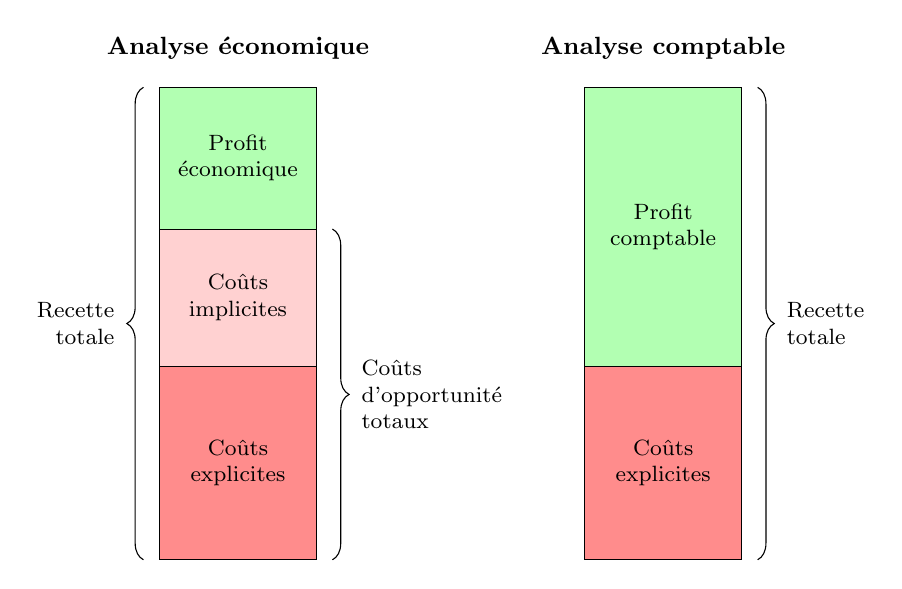
\begin{tikzpicture}[font=\footnotesize,
      blk/.style={draw,align=center},
      brc/.style={decorate,decoration={brace,amplitude=6pt}}]
    % economist's bar
    \draw[blk,fill=red!45] (0,0) rectangle (2,2.46);
    \draw[blk,fill=red!18] (0,2.46) rectangle (2,4.2);
    \draw[blk,fill=green!30] (0,4.2) rectangle (2,6);
    \node[align=center] at (1,1.23) {Coûts\\explicites};
    \node[align=center] at (1,3.33) {Coûts\\implicites};
    \node[align=center] at (1,5.1) {Profit\\économique};
    \node[align=center,font=\small\bfseries] at (1,6.5) {Analyse économique};
    \draw[brc] (-0.2,0) -- (-0.2,6)
      node[midway,left=7pt,align=right] {Recette\\totale};
    \draw[brc] (2.2,4.2) -- (2.2,0)
      node[midway,right=7pt,align=left] {Coûts\\d'opportunité\\totaux};
    % accountant's bar
    \draw[blk,fill=red!45] (5.4,0) rectangle (7.4,2.46);
    \draw[blk,fill=green!30] (5.4,2.46) rectangle (7.4,6);
    \node[align=center] at (6.4,1.23) {Coûts\\explicites};
    \node[align=center] at (6.4,4.23) {Profit\\comptable};
    \node[align=center,font=\small\bfseries] at (6.4,6.5) {Analyse comptable};
    \draw[brc] (7.6,6) -- (7.6,0)
      node[midway,right=7pt,align=left] {Recette\\totale};
  \end{tikzpicture}
  \caption*{\small Analyse économique contre analyse comptable. One recette totale,
  split two ways: the economist subtracts all the coûts d'opportunité, the
  accountant only the coûts explicites, so the profit économique is the smaller of
  the two profits.}
\end{figure}

\subsection{Coût moyen et coût marginal}

Everything starts from the coût total. The symbols are the English initials the
course uses.

\begin{definition}[Coût total (\textit{total cost})]
  Coût total $(TC)$ = Coût fixe $(FC)$ + coût variable $(VC)$.
\end{definition}
That is, $TC = FC + VC$: the coût total splits into the \textbf{coût fixe}
(\textit{fixed cost}) $FC$ and the \textbf{coût variable} (\textit{variable cost})
$VC$. The two costs of the title are built from it.

\begin{definition}[Coût moyen (\textit{average total cost}) et coût marginal (\textit{marginal cost})]
  \[ ATC = \frac{TC}{Q}, \qquad MC = \frac{\Delta TC}{\Delta Q}. \]
\end{definition}
In words: the coût moyen is the coût total divided by the quantity $Q$, and the
coût marginal is the change in the coût total divided by the change in quantity,
$\Delta$ standing for a change.\\

The figure draws the cost curves of a typical firm: $MC$ and $ATC$, and two
curves the definitions above do not give, $AVC$, the curve of the
\textbf{coût variable moyen} (\textit{average variable cost}), and $AFC$, that of
the \textbf{coût fixe moyen} (\textit{average fixed cost}). Many firms have a
\textbf{produit marginal} (\textit{marginal product}) that is increasing at first
and then diminishing. As a result their cost curves have the shapes of the figure:
the coût marginal and the coût variable moyen fall for a while before starting to
rise. As drawn, moreover:
\begin{itemize}
  \item the rising $MC$ passes through the minimum of $AVC$, then through the
    minimum of $ATC$;
  \item $ATC$ lies above $AVC$, the gap between them at each quantity being the
    height of $AFC$, and the gap narrows as the quantity grows;
  \item $AFC$ falls throughout.
\end{itemize}

\begin{figure}[h!]
  \centering
  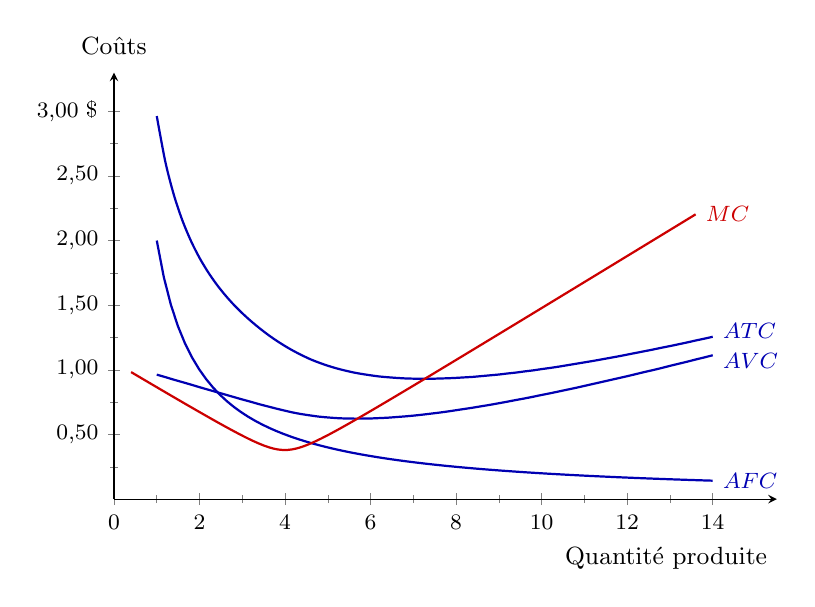
\begin{tikzpicture}
    \begin{axis}[
        width=10cm, height=7cm,
        axis lines=left,
        xmin=0, xmax=15.5, ymin=0, ymax=3.3,
        xtick={0,2,...,14},
        minor xtick={1,3,...,13},
        ytick={0.5,1,1.5,2,2.5,3},
        yticklabels={$0{,}50$,$1{,}00$,$1{,}50$,$2{,}00$,$2{,}50$,$3{,}00$~\$},
        minor ytick={0.25,0.75,...,2.75},
        tick label style={font=\footnotesize},
        xlabel={Quantité produite}, ylabel={Coûts},
        xlabel style={at={(axis description cs:1,-0.09)},anchor=north east,font=\small},
        ylabel style={at={(axis description cs:0,1.02)},rotate=-90,anchor=south,font=\small},
        clip=false,
      ]
      % AFC = FC/Q with FC = 2
      \addplot[blue!70!black,thick,domain=1:14,samples=80] {2/x}
        node[right,font=\footnotesize] {$AFC$};
      % AVC and ATC: VC is the integral of MC, FC = 2
      \addplot[blue!70!black,thick,smooth] coordinates {
        (1.00,0.963) (1.20,0.944) (1.40,0.924) (1.60,0.905) (1.80,0.886) (2.00,0.866)
        (2.20,0.847) (2.40,0.828) (2.60,0.809) (2.80,0.790) (3.00,0.771) (3.20,0.753)
        (3.40,0.734) (3.60,0.717) (3.80,0.700) (4.00,0.684) (4.20,0.669) (4.40,0.657)
        (4.60,0.647) (4.80,0.638) (5.00,0.632) (5.20,0.627) (5.40,0.624) (5.60,0.623)
        (5.80,0.623) (6.00,0.624) (6.20,0.627) (6.40,0.630) (6.60,0.635) (6.80,0.640)
        (7.00,0.646) (7.20,0.653) (7.40,0.661) (7.60,0.669) (7.80,0.678) (8.00,0.688)
        (8.20,0.698) (8.40,0.708) (8.60,0.719) (8.80,0.730) (9.00,0.742) (9.20,0.754)
        (9.40,0.767) (9.60,0.779) (9.80,0.792) (10.00,0.806) (10.20,0.819) (10.40,0.833)
        (10.60,0.847) (10.80,0.861) (11.00,0.876) (11.20,0.891) (11.40,0.906) (11.60,0.921)
        (11.80,0.936) (12.00,0.951) (12.20,0.967) (12.40,0.983) (12.60,0.998) (12.80,1.014)
        (13.00,1.031) (13.20,1.047) (13.40,1.063) (13.60,1.080) (13.80,1.096) (14.00,1.113)}
        node[right,font=\footnotesize,yshift=-2pt] {$AVC$};
      \addplot[blue!70!black,thick,smooth] coordinates {
        (1.00,2.963) (1.20,2.610) (1.40,2.353) (1.60,2.155) (1.80,1.997) (2.00,1.866)
        (2.20,1.756) (2.40,1.661) (2.60,1.578) (2.80,1.504) (3.00,1.438) (3.20,1.378)
        (3.40,1.323) (3.60,1.272) (3.80,1.226) (4.00,1.184) (4.20,1.146) (4.40,1.112)
        (4.60,1.081) (4.80,1.055) (5.00,1.032) (5.20,1.012) (5.40,0.995) (5.60,0.980)
        (5.80,0.968) (6.00,0.958) (6.20,0.949) (6.40,0.943) (6.60,0.938) (6.80,0.934)
        (7.00,0.932) (7.20,0.931) (7.40,0.931) (7.60,0.933) (7.80,0.935) (8.00,0.938)
        (8.20,0.942) (8.40,0.946) (8.60,0.952) (8.80,0.958) (9.00,0.964) (9.20,0.972)
        (9.40,0.979) (9.60,0.988) (9.80,0.996) (10.00,1.006) (10.20,1.015) (10.40,1.025)
        (10.60,1.036) (10.80,1.047) (11.00,1.058) (11.20,1.069) (11.40,1.081) (11.60,1.093)
        (11.80,1.105) (12.00,1.118) (12.20,1.131) (12.40,1.144) (12.60,1.157) (12.80,1.171)
        (13.00,1.184) (13.20,1.198) (13.40,1.212) (13.60,1.227) (13.80,1.241) (14.00,1.256)}
        node[right,font=\footnotesize,yshift=2pt] {$ATC$};
      % MC
      \addplot[red!80!black,thick,domain=0.4:13.6,samples=120]
        {0.26+0.002*(x-4)+sqrt((0.2*(x-4))^2+0.0144)}
        node[right,font=\footnotesize] {$MC$};
    \end{axis}
  \end{tikzpicture}
  \caption*{\small Courbes de coûts d'une entreprise type. The coût marginal and
  the coût variable moyen first fall, then rise; the rising $MC$ crosses $AVC$ and
  then $ATC$ at their minima, and $AFC$ falls throughout.}
\end{figure}

\subsection{Rendements d'échelle}

The \textbf{rendements d'échelle} (\textit{returns to scale}) are read off a single
figure, which sets the coût moyen à \textbf{court terme} (\textit{short run})
against the coût moyen à long terme. Because the coûts fixes are variable à long
terme, the $ATC$ curve à court terme differs from the $ATC$ curve à long terme. The
figure draws three $ATC$ curves à court terme, for a small, a medium and a large
factory, and the $ATC$ curve à long terme, which lies on or below each of them and
touches each once. Along the curve à long terme, three stretches are named:
\begin{itemize}
  \item where it falls, \textbf{économies d'échelle} (\textit{economies of scale});
  \item where it is flat, here at 10\,000, \textbf{rendements d'échelle constants}
    (\textit{constant returns to scale});
  \item where it rises, \textbf{déséconomies d'échelle}
    (\textit{diseconomies of scale}).
\end{itemize}
The figure also marks two quantities. At 1\,000 cars per day, the medium
factory's $ATC$ à court terme is at its minimum, 10\,000, on the curve à long terme.
At 1\,200 cars per day it has risen to 12\,000~\$, while the $ATC$ à long terme
is still 10\,000.

\begin{figure}[h!]
  \centering
  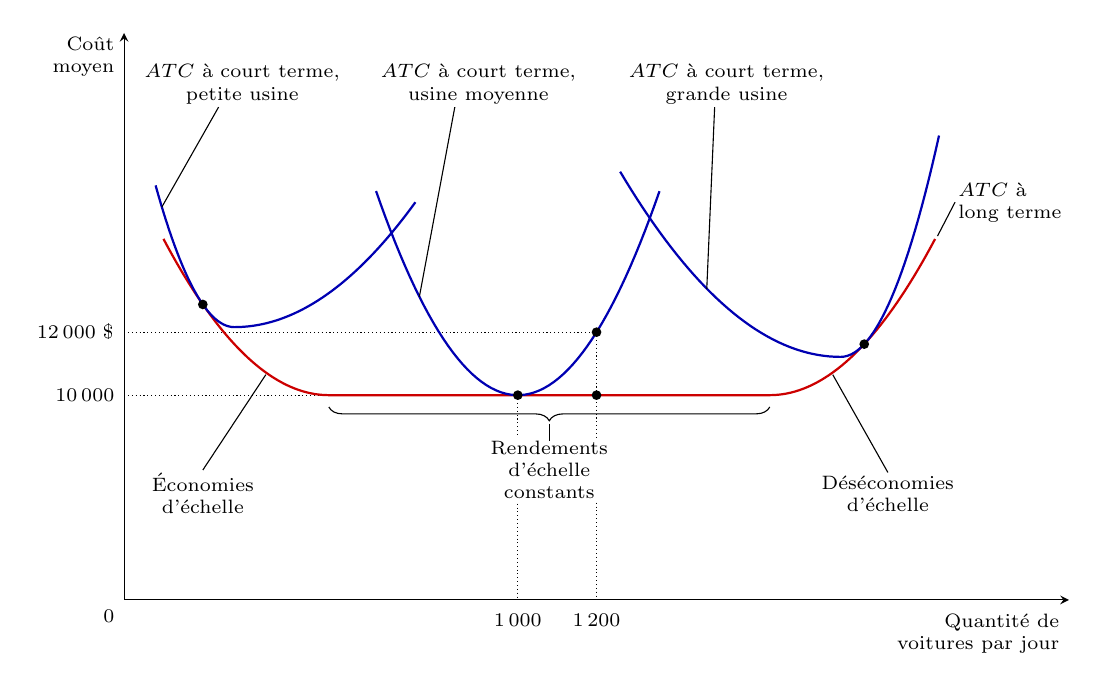
\begin{tikzpicture}[font=\scriptsize,>=stealth,
      sr/.style={blue!70!black,thick},
      lr/.style={red!80!black,thick},
      lab/.style={align=center,inner sep=1pt},
      dot/.style={circle,fill=black,inner sep=0pt,minimum size=3.5pt}]
    % axes
    \draw[->] (0,0) -- (12,0);
    \draw[->] (0,0) -- (0,7.2);
    \node[below left] at (0,0) {$0$};
    \node[left,align=right] at (0,6.9) {Coût\\moyen};
    \node[below left,align=right] at (12,-0.05) {Quantité de\\voitures par jour};
    % guides
    \draw[densely dotted] (0,3.4) -- (6,3.4);
    \draw[densely dotted] (0,2.6) -- (2.6,2.6);
    \draw[densely dotted] (5,2.6) -- (5,0);
    \draw[densely dotted] (6,3.4) -- (6,0);
    \node[left] at (0,3.4) {$12\,000$~\$};
    \node[left] at (0,2.6) {$10\,000$};
    \node[below] at (5,-0.05) {$1\,000$};
    \node[below] at (6,-0.05) {$1\,200$};
    % long-run ATC
    \draw[lr] plot[domain=0.5:2.6,samples=40] (\x,{2.6+0.45*(2.6-\x)^2})
      -- (8.2,2.6)
      -- plot[domain=8.2:10.3,samples=40] (\x,{2.6+0.45*(\x-8.2)^2});
    % short-run ATC: small, medium, large factory
    \draw[sr] plot[domain=0.4:1.4,samples=30] (\x,{3.464+1.8*(\x-1.4)^2})
      -- plot[domain=1.4:3.7,samples=40] (\x,{3.464+0.3*(\x-1.4)^2});
    \draw[sr] plot[domain=3.2:6.8,samples=60] (\x,{2.6+0.8*(\x-5)^2});
    \draw[sr] plot[domain=6.3:9.1,samples=40] (\x,{3.086+0.3*(\x-9.1)^2})
      -- plot[domain=9.1:10.35,samples=30] (\x,{3.086+1.8*(\x-9.1)^2});
    % points
    \foreach \p in {(1.0,3.752),(5,2.6),(6,3.4),(6,2.6),(9.4,3.248)}
      \node[dot] at \p {};
    % curve labels
    \node[lab] (s) at (1.5,6.55) {$ATC$ à court terme,\\petite usine};
    \draw (s.south) ++(-0.3,0) -- (0.48,4.99);
    \node[lab] (m) at (4.5,6.55) {$ATC$ à court terme,\\usine moyenne};
    \draw (m.south) ++(-0.3,0) -- (3.75,3.85);
    \node[lab] (g) at (7.65,6.55) {$ATC$ à court terme,\\grande usine};
    \draw (g.south) ++(-0.15,0) -- (7.4,3.95);
    \node[lab,align=left] (l) at (11.25,5.05) {$ATC$ à\\long terme};
    \draw (l.west) -- (10.33,4.62);
    % stretches of the long-run curve
    \draw[decorate,decoration={brace,amplitude=5pt}] (8.2,2.45) -- (2.6,2.45);
    \node[lab,fill=white] at (5.4,1.65) {Rendements\\d'échelle\\constants};
    \draw (5.4,2.24) -- (5.4,2.02);
    \node[lab] (e) at (1.0,1.35) {Économies\\d'échelle};
    \draw (e.north) -- (1.8,2.86);
    \node[lab] (d) at (9.7,1.35) {Déséconomies\\d'échelle};
    \draw (d.north) -- (9.0,2.86);
  \end{tikzpicture}
  \caption*{\small Coût moyen à court terme et à long terme. The $ATC$ curve à long
  terme lies on or below the three curves à court terme and touches each once; it
  falls, is flat, then rises. At 1\,200 cars per day the medium factory's
  $ATC$ à court terme is 12\,000~\$, the $ATC$ à long terme still 10\,000.}
\end{figure}

\subsection{Équilibre de long terme}

The last figure puts the cost curves to work for a competitive firm. À long terme,
the firm's \textbf{courbe d'offre de long terme} (\textit{long-run supply curve})
is its $MC$ curve above $ATC$; if the price falls below $ATC$, the firm is better
off leaving the market. The figure draws that supply as a thick line, in two
pieces:
\begin{enumerate}
  \item the part of $MC$ above the minimum of $ATC$: à long terme, the firm
    produces on the $MC$ curve if $P > ATC$;
  \item the part of the vertical axis below that minimum: the firm exits if
    $P < ATC$, and supplies nothing.
\end{enumerate}
The part of $MC$ below the minimum of $ATC$, drawn pale, is not part of the supply.
This closes the loop with the chapter's opening claim: à long terme, what the
competitive firm supplies is read off its structure des coûts.

\begin{figure}[h!]
  \centering
  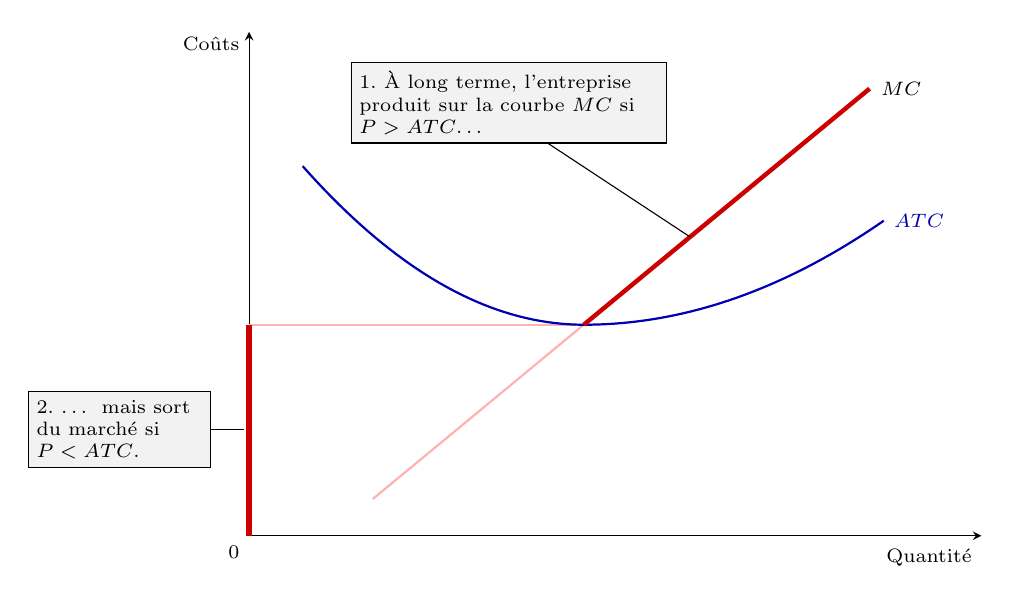
\begin{tikzpicture}[font=\scriptsize,>=stealth,
      call/.style={draw,fill=black!5,align=left,inner sep=3pt}]
    % axes
    \draw[->] (0,0) -- (9.3,0);
    \draw[->] (0,0) -- (0,6.4);
    \node[below left] at (0,0) {$0$};
    \node[left] at (0,6.25) {Coûts};
    \node[below left] at (9.3,-0.05) {Quantité};
    % pale parts: MC below the minimum of ATC, guide at that minimum
    \draw[red!30,thick] (0,2.68) -- (4.25,2.68);
    \draw[red!30,thick] (1.57,{2.68+0.826*(1.57-4.25)}) -- (4.25,2.68);
    % ATC
    \draw[blue!70!black,thick] plot[domain=0.68:4.25,samples=40] (\x,{2.68+0.158*(\x-4.25)^2})
      -- plot[domain=4.25:8.06,samples=40] (\x,{2.68+0.091*(\x-4.25)^2})
      node[right] {$ATC$};
    % supply: MC above the minimum of ATC, and the axis below it
    \draw[red!80!black,line width=1.6pt] (4.25,2.68) -- (7.88,{2.68+0.826*(7.88-4.25)})
      node[right,text=black] {$MC$};
    \draw[red!80!black,line width=2.4pt] (0,0) -- (0,2.68);
    % callouts
    \node[call,text width=3.8cm] (c1) at (3.3,5.5)
      {1.\ À long terme, l'entreprise produit sur la courbe $MC$ si ${P > ATC}$\ldots};
    \draw (c1.south) ++(0.5,0) -- (5.6,{2.68+0.826*(5.6-4.25)});
    \node[call,text width=2.1cm] (c2) at (-1.65,1.35)
      {2.\ \ldots{} mais sort du marché si ${P < ATC}$.};
    \draw (c2.east) -- (-0.06,1.35);
  \end{tikzpicture}
  \caption*{\small Courbe d'offre de long terme de l'entreprise concurrentielle.
  The thick line is the supply: $MC$ above the minimum of $ATC$, and nothing
  produced at prices below that minimum.}
\end{figure}
